\documentclass[sigconf]{acmart}

\usepackage{graphicx}
\usepackage{hyperref}
\usepackage{todonotes}

\usepackage{endfloat}
\renewcommand{\efloatseparator}{\mbox{}} % no new page between figures

\usepackage{booktabs} % For formal tables

\settopmatter{printacmref=false} % Removes citation information below abstract
\renewcommand\footnotetextcopyrightpermission[1]{} % removes footnote with conference information in first column
\pagestyle{plain} % removes running headers

\newcommand{\TODO}[1]{\todo[inline]{#1}}

\begin{document}

\title{Big Data Analytics and IoT Smart Refridgerators}


\author{Robert W. Gasiewicz}
\orcid{1234-5678-9012}
\affiliation{%
  \institution{Indiana University}
  \streetaddress{711 N. Park Avenue}
  \city{Bloomington} 
  \state{IN} 
  \postcode{47408}
}
\email{rgasiewi@iu.edu}

\begin{abstract}

The intent of this paper is to explore the rapid growth of IoT Smart Appliances, specifically with regard to refrigerators. As more devices are connected to the internet, to each other, and become readily available to consumers, there are many exciting new possibilities that offer both convenience and to make our lives more efficient. The scope of this paper will begin with a brief history of IoT, then move on to describe the current way in which this technology is being applied, and conclude with exploration and outlook on future development possibilities as well as potential risks. 

\end{abstract}

\keywords{i523, HID316, Big Data, IoT, Refrigerators, Smart Appliances, M2M, Samsung, Innit, Instacart, GrubHub}

\maketitle

\section{Introduction}

The advent of the Internet of Things (IoT) began at the close of the last millennium when the world began connecting ordinary devices - electronics other than traditional computers - to the internet. With virtually unlimited possibilities, the unthinkable became reality when the concept of putting a wireless network card in a refrigerator went mainstream. Initial features were as simple as a large touchscreen with the news, the weather, and a doodle board. 
\par
From there, IoT Smart Refrigerators have evolved to become equipped with cameras, cooking recommendations, and even rudimentary food inventory and spoilage management systems. Now that food delivery services such as Instacart and GrubHub have become popular, there are already plans to integrate these services with smart refrigerators. As IoT has continued to expand throughout the marketplace and the concept of machine-to-machine (M2M) IoT has taken hold, there are now even more possibilities, which means a bright future in the kitchen no matter if you're an aspiring chef, a person trying to efficiently manage a family, or someone with specific health needs. However, along with the rapid advance of new features, there are also significant threats and blind spots with security. 

\section{Early History of IoT and Networked Appliances}

Although the internet didn't yet exist in the minds of Hollywood producers in 1985, the opening scene from Back to the Future begins with a room full of ticking clocks, one of which is an alarm clock that rings and sets off a Rube Goldberg machine that has been configured by Doc Brown to automate the preparation of his breakfast. It's not unreasonable to believe that, in his many time travel escapades, Doc would've eventually "discovered" the internet and would've upgraded this rudimentary appliance. 
\par
That reality wouldn't come until five years later in 1990 when the first IoT device, a toaster, was turned off and on via the internet. At the October 1989 INTEROP Conference, John Ramkey used a Sunbeam Radiant Control toaster connected to a TCP/IP network to demonstrate that the device could be turned off and on\cite{Ramkey01}. Not only did Ramkey succeed at turning the toaster on and off, he used SNMP code delivered via his computer's parallel port to a larger relay to control power to the toaster. The SNMP code executed commands for a value, 1 through 10, for the toast's doneness as well as a calculation for the type of item being toasted. For example, while the command for wheat bread would tell the toaster to toast at a level of 2, the command for a frozen bagel would tell the toaster to toast at a level of 5. Additional innovations were later added, such as a Lego robotic arm to insert the bread into the toaster; a sight Doc Brown would've been proud to see.
\par
By 1999, the Salt Lake City Tribune/Deseret News was predicting that household appliances like the refrigerator were going to be part of a future in which "everyone lived like the Jetsons"\cite{Deseret1999}. "The networked home is on the horizon", the Tribune/Deseret News' Michael Stroh wrote, "with a click, you call up your refrigerator on your office PC to see what's inside (a bar-code reader within the fridge keeps a running inventory). The refrigerator suggests lasagna but warns that you'll need to buy ricotta - and a few other items."\cite{Deseret1999} Not surprisingly, it would be at least another decade before this concept became a viable reality. 

\section{IoT is Born}

The first time the term "Internet of Things" was used wasn't until nine years later by Kevin Ashton, co-founder of the Auto-ID Center at the Massachusetts Institute of Technology (MIT). The Auto-ID Center was founded with the expressed purpose of creating a formal standard for Radio Frequency Identification (RFID) and other types of networked sensors. In 2009, Kevin wrote\cite{Ashton01}: "I could be wrong, but I'm fairly sure the phrase "Internet of Things" started life as the title of a presentation I made at Procter \& Gamble (P\&G) in 1999. Linking the new idea of RFID in P\&G's supply chain to the then-red-hot topic of the Internet was more than just a good way to get executive attention. It summed up an important insight which is still often misunderstood."
\par
Even though Kevin briefly captured the momentary attention of the C-Suite at P\&G, it wasn't another full decade until the true concept of IoT caught on in the marketplace. In 2011, the market research company Gartner, included IoT on their hype cycle chart for the very first time. By 2016, IoT was past-peak of inflated expectations was doing the usual nosedive into the trough of disillusionment\cite{Gartner2017}.

\begin{figure}
  \TODO{image missing}
  %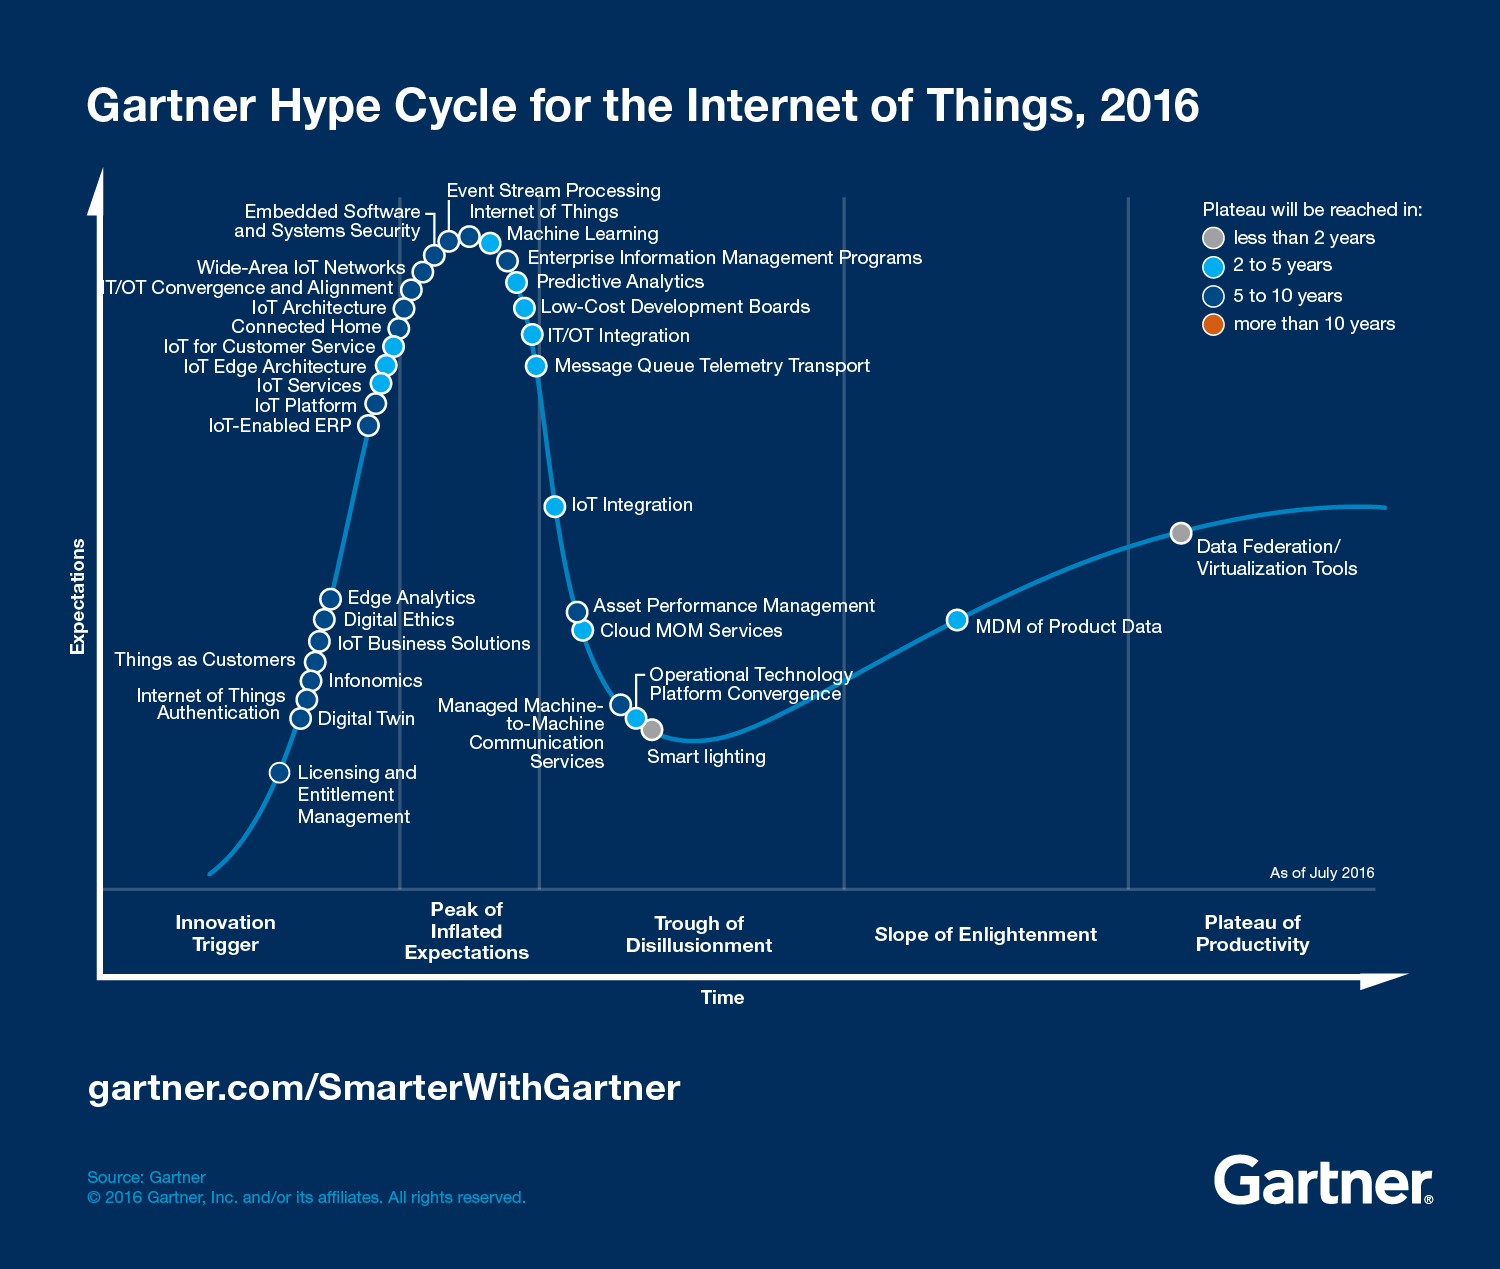
\includegraphics[width=\linewidth]{gartner2016.png}
  \caption{2016 Gartner Hype-Cycle Chart.}
  \label{fig:Gartner2016}
\end{figure}

\section{IoT Smart Refrigerators Come of Age}

Internet refrigerators, on the other hand were a bit slower catching up. After many failed attempts in the mid-2000s at various gimmicky models, it seemed that the once rosy future painted by Mr. Stroh a decade earlier was simply not going to come to fruition. Hardware and network technology had not yet caught up. By 2014, murmurs of a new wave of internet fridges hit the marketplace and excitement began to build, and by 2016, the IoT Refrigerator was ready for primetime. On January 24, 2016, Samsung launched its Smart Hub Refrigerator complete with a massive 21.5 inch 1080P touchscreen and Android operating system. Another exciting new feature of the Smart Hub fridge was the interior cameras that allowed users to get a real-time look at the contents of their fridge from anywhere\cite{PocketLint2016}.
\par
A year later, Samsung debuted version 2.0 of the Smart Hub fridge, this time with improvements such as third-party apps such as Spotify and individualized user profiles for family members. Users are also able to serve photos and other content to the screen as well. Interestingly, Samsung has opted to go with the its own proprietary voice control system called S-Voice, while its only current competitor in the IoT fridge marketplace, LG, will integrate with Amazon's Alexa. Only in Europe, with the LidL supermarket chain, will consumers be able to order groceries through the the fridge. It's a start, but there is much, much more on the horizon\cite{PocketLint2017}.

\section{The Future of IoT Smart Refrigerators}

The future of IoT Smart Refrigerators - and kitchen appliances working in concert in general - is brighter than perhaps Doc Brown or even John Ramkey could have ever imagined. Hardware, networking, and most importantly, software, have all caught up to be viable in fulfilling consumer demands and there are fresh new ideas already just beginning to hit the marketplace. The next phase of the IoT Smart Refrigerator will be one that is marked by progress in software. Structurally speaking, refrigerators are designed to last between 14-17 years\cite{SFGate2017}, however, the average consumer might upgrade their personal computer 3 to 4 times during this time span. In other words, an IoT Smart Refrigerator made today, might only be 1/4 to 1/3 of the way through its average lifespan before its computer and networking components become obsolete. 
\par
One Silicon Valley company that seems to have a viable solution to this problem is Innit\cite{Innit2017}. Innit has come up with the idea of having a cloud-based platform for the kitchen that partners with appliance manufacturers such as Jenn Air and Whirlpool to add their components and integrate their application with existing appliance platforms. The idea is that you can equip your entire kitchen, not just the refrigerator, with technology that can make anyone a culinary master with a bit of guidance\cite{CNBC2017}. Building upon Samsung's successful Smart Hub fridge platform, Innit takes the camera-in-your-fridge concept a step further by introducing image recognition software that can be used to interface with the cloud to generate recipes based on available ingredients, manage spoilage, and inventory - including placing orders for new food. The technology would also enable other kitchen appliances such as an oven or microwave to interact with one another to create a meal. 
\par
Aside from personal convenience, one of the most significant values derived from the advance of this sort of technology is that it could prevent an enormous amount of food waste. The United Nations' Food and Agriculture Organization estimates that up to 1.3 billion tons of food are wasted globally every year\cite{FAO2017}, which equates to roughly 30 percent of all food produced in the same time-frame.  Ultimately, software like Innit's because it is connected to the cloud and utilizing big data to allow consumers to make informed decisions about what they eat, people will live and eat healthier and greener.  

\section{Smart and Dangerous: An IoT Double-Edged Sword}

Yes - it is true - both today and in the future, your IoT Smart Refrigerator will help you live better, but as Swapnil Bhartiya points out in a recent article on InfoWorld\cite{Bhartiya2017}, it could also kill you. It sounds ominous, but the rapid growth of IoT comes with a steep price: lack of security. Consumers can never really be sure if their software will be patched properly and for how long. It has been well-documented that hackers have been able to successfully commandeer smart devices and utilize them to aggressively launch DDoS that disabled a sizeable portion of the internet. An even bigger threat is that, once compromised, a vulnerable smart device will work as a Trojan Horse allowing nefarious users to access other devices on your local network. Once you throw Alexa into the mix, all bets are off. 
\par
One development that is offsetting this risk is the unification of IoT networks in the cloud. Samsung is now creating a SmartThings cloud in which all of its IoT devices will interact. This centraliztion makes security and big data much easier to manage. This unification is also occurring at the macro level with Cisco and Google's cloud\cite{Cisco2017} which will hopes to achieve the following goals:

\begin{enumerate}
  \item Freedom to access any resource while preserving security and compliance
  \item Ability to extend policy to cloud environments to optimize applications
  \item Extend visibility, threat detection and control across hybrid environments without slowing innovation
\end{enumerate}

\section{Conclusion}

IoT has a very bright future ahead and the rapidly evolving IoT Smart Refrigerator will serve as the centerpiece not only to a smart, connected kitchen, but to a smart, connected, and secure home. While it was hardware and networking that delayed progress in the 1990s and software and implementation that led to stagnation in the 2000s, security serves as the next challenge to be overcome as IoT Smart Refrigerators join the burgeoning global network of IoT smart devices.

\bibliographystyle{ACM-Reference-Format}
\bibliography{report} 

\end{document}
